\documentclass[12 pt,twoside]{article}
\usepackage{epsfig}
\usepackage{fullpage}
\usepackage[font={small,it}]{caption}

\begin {document}
\begin{center}

{\LARGE{\bf Broadband Imaging and Photometry on Open Star Clusters}}

{\large Tim Kornish}

University of Montana

November 24th, 2014
\end{center}

\paragraph{Abstract}

\paragraph{Introduction}

\paragraph{Observations}

\ \

observing NGC 1234 with 0.4m telescope at U of M. 

\ \

Using R fro 5 seconds, V 5 seconds, B 10 seconds filters to produce a color magnitude image of the open star cluster

\ \

Sept 2


\paragraph{Methods}

\paragraph{Analysis}

Create Mosaic image due to dithering

\ \

\begin{center}
\begin{figure}[!hb]
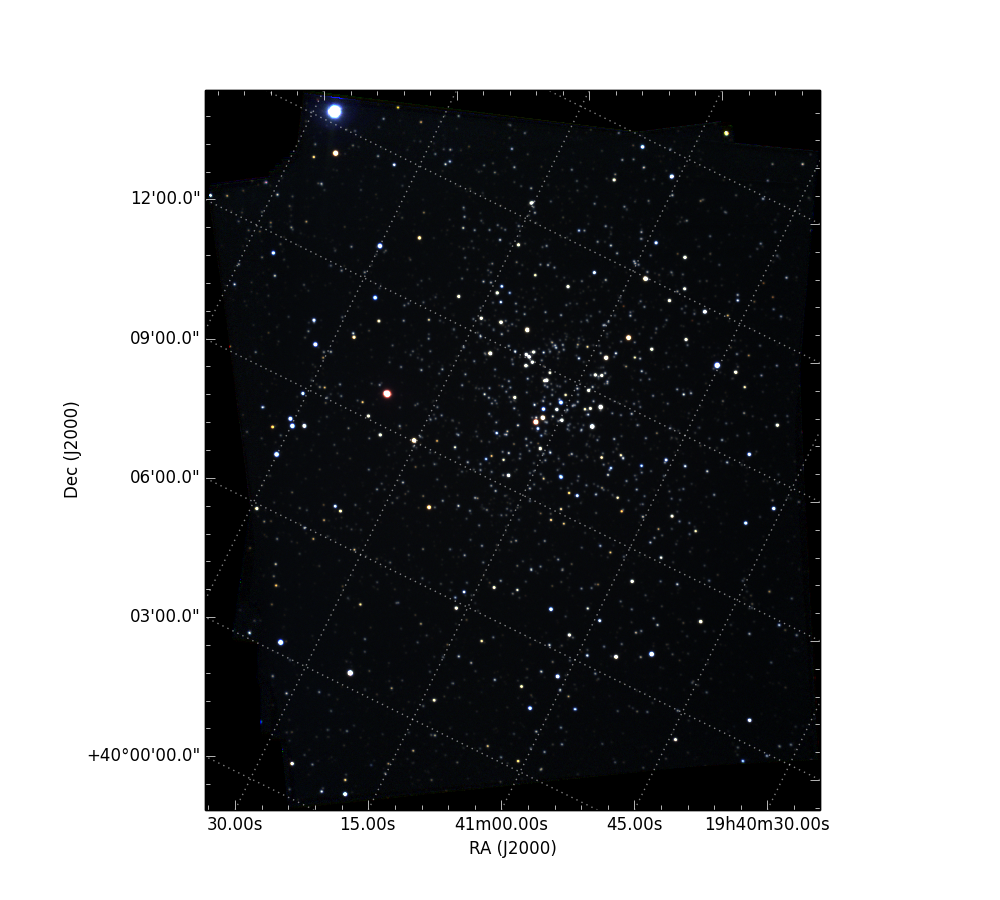
\includegraphics[scale=0.7]{figure_1.png}
\caption{\small{shows an x-axis of 10 data samples ranging 0-9 and y-axis being the number of photons counted in the 10ms interval. with a {\it mean} = 19 photons, $\sigma$ = 8.68 }}
\end{figure}
\end{center}

\begin{center}
\begin{figure}[!hb]
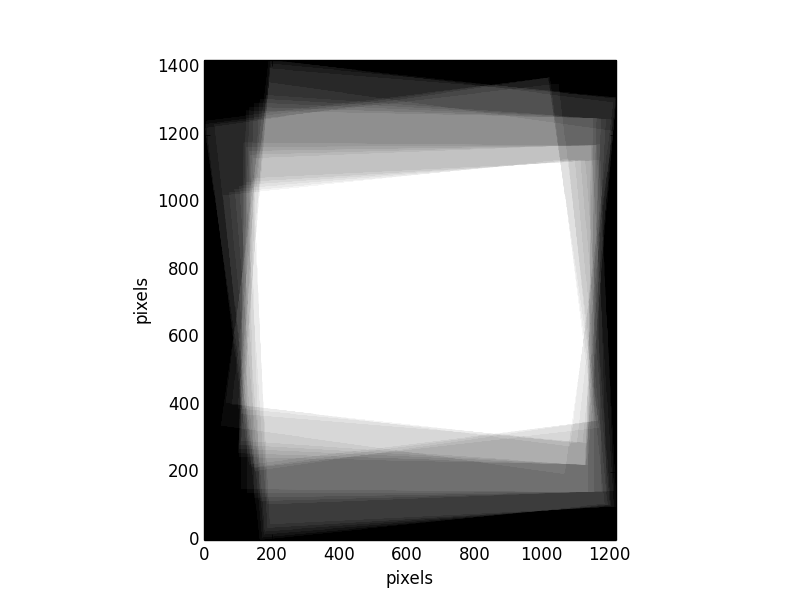
\includegraphics[scale=0.7]{figure_2.png}
\caption{\small{shows an x-axis of 10 data samples ranging 0-9 and y-axis being the number of photons counted in the 10ms interval. with a {\it mean} = 19 photons, $\sigma$ = 8.68 }}
\end{figure}
\end{center}

\begin{center}
\begin{figure}[!hb]
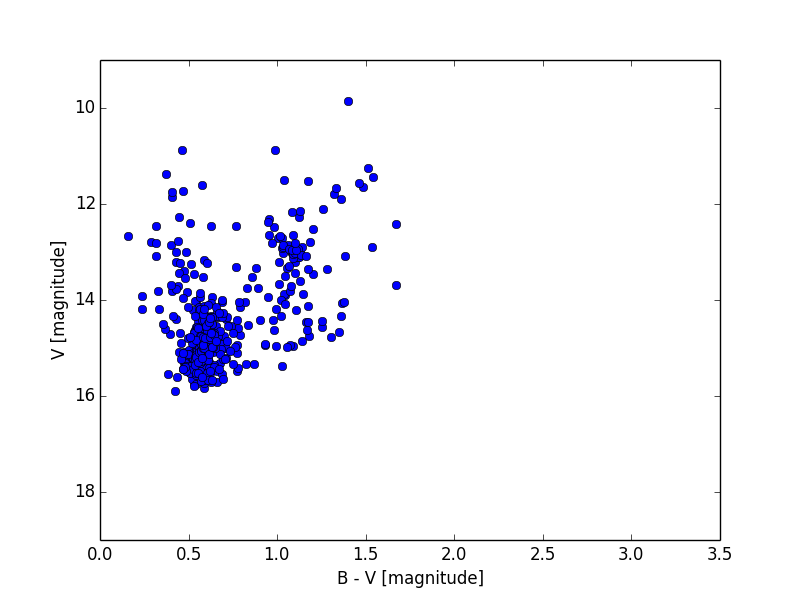
\includegraphics[scale=0.7]{figure_3.png}
\caption{\small{shows an x-axis of 10 data samples ranging 0-9 and y-axis being the number of photons counted in the 10ms interval. with a {\it mean} = 19 photons, $\sigma$ = 8.68 }}
\end{figure}
\end{center}

\paragraph{Results}

\paragraph{Concusion}




















\end{document}